% 第4章第6节：随机概率测度（随机质量、评价σ代数、Dirichlet分布、折棒构造与Dirichlet过程）。

\section{随机概率测度}
\label{sec:spp-random-measures}

de Finetti定理中的随机背景$\Xi$是一个随机的概率分布。若要直接为这样的背景建模，例如事先不假定总体属于某个参数族，而是让整个总体分布随机，就需要一种构造随机概率测度的方法。本节的索引是可测集合：每个集合$A$得到一个随机质量$G(A)$。集合之间没有时间顺序，离散与连续时间的区分在这里不适用；新的要求是，每次实现都必须是一个真正的概率测度。我们先说明随机概率测度的准确含义及它与几种相近对象的区别，再用折棒构造得到Dirichlet过程，并证明它在有限分割上的质量服从Dirichlet分布。

\subsection{集合上的随机质量}
\label{sec:spp-random-mass}

\paragraph{随机离散测度}
最直接的随机概率测度由随机权重和随机位置组成。设$w_1,w_2,\ldots$是非负随机变量，几乎必然满足$\sum_kw_k=1$；$\xi_1,\xi_2,\ldots$是取值于$(E,\mathcal E)$的随机变量。令
\begin{equation}
  G(A)=\sum_{k=1}^\infty w_k\,\mathbb I_A(\xi_k),\qquad A\in\mathcal E .
  \label{eq:spp-random-discrete}
\end{equation}
它是在随机位置$\xi_k$上放置随机质量$w_k$的离散测度。对固定的$\omega$（在$\sum_kw_k=1$成立的事件上），$A\mapsto G(A)$是概率测度：$G(E)=\sum_kw_k=1$，并且对两两不交的$A_1,A_2,\ldots$，非负项级数可以交换求和次序，
\[
  G\Bigl(\bigcup_jA_j\Bigr)=\sum_kw_k\sum_j\mathbb I_{A_j}(\xi_k)=\sum_j\sum_kw_k\mathbb I_{A_j}(\xi_k)=\sum_jG(A_j).
\]
对固定的$A$，$G(A)$是可数个随机变量之和，因而是随机变量。图~\ref{fig:spp-random-measure-partition}(a)画出一次实现：竖线的位置是原子$\xi_k$，高度是权重$w_k$；(b)把$[0,1]$分成三段，每段的质量就是落在其中的竖线高度之和。

\begin{figure}[htbp]
  \centering
  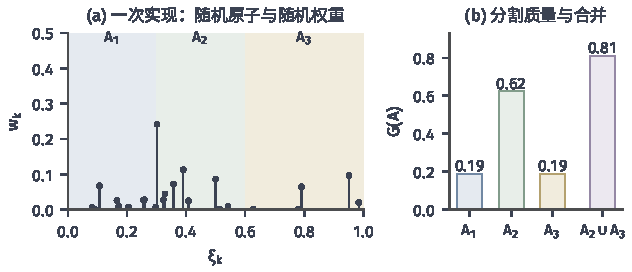
\includegraphics[width=107mm]{figures/03-optimization-evolution-and-signals/02-processes-and-trajectory-evolution/matplotlib/spp-random-measure-partition/figure.pdf}
  \caption{一个随机离散概率测度的一次实现。原子$\xi_k$独立服从$[0,1]$上的均匀分布，权重$w_k$由浓度参数$\alpha=5$的折棒构造产生（第~\ref{sec:spp-dirichlet-process}小节），共生成$400$个原子，图(a)只画出权重大于$10^{-3}$者（固定随机种子）。(b)分割$A_1=[0,0.3)$、$A_2=[0.3,0.6)$、$A_3=[0.6,1]$上的质量，以及合并$A_2\cup A_3$后的质量：合并分块时质量相加。}
  \label{fig:spp-random-measure-partition}
\end{figure}

\paragraph{评价$\sigma$代数与随机概率测度}
要把“随机的概率测度”当作一个随机对象，需要在概率测度的集合上规定$\sigma$代数。记$\mathcal P(E)$为$(E,\mathcal E)$上全体概率测度。对每个$A\in\mathcal E$，评价映射$\operatorname{ev}_A:\nu\mapsto\nu(A)$把一个概率测度映为一个数。使所有评价映射可测的最小$\sigma$代数称为\term{评价$\sigma$代数}（evaluation sigma-algebra）。

\begin{definition}[随机概率测度]
\label{def:spp-random-probability-measure}
从概率空间$(\Omega,\mathcal F,\mathbb P)$到$\mathcal P(E)$（配评价$\sigma$代数）的可测映射$G$称为$E$上的随机概率测度。
\end{definition}

这个定义可以逐个集合检查：$G$可测，当且仅当对每个$A\in\mathcal E$，$\omega\mapsto G(\omega)(A)$是随机变量。必要性是因为$\operatorname{ev}_A\circ G$是可测映射的复合；充分性的论证与定理~\ref{thm:spp-path-law}(1)相同，因为评价$\sigma$代数由集合$\operatorname{ev}_A^{-1}(B)$生成，而它们的原像$\{G(A)\in B\}$都属于$\mathcal F$。按此判据，式~\eqref{eq:spp-random-discrete}在零概率例外事件上另行指定为某个固定的概率测度后，就是一个随机概率测度。

\paragraph{三类对象的区别}
随机概率测度容易与几种相近对象混淆，它们的随机性来源与极限行为不同。

第一类是固定总体的\term{经验测度}（empirical measure）。设$X_1,X_2,\ldots$独立同分布于固定的概率测度$\nu$，$\nu_n=\frac1n\sum_{i=1}^n\delta_{X_i}$。$\nu_n$也是随机概率测度，但它的随机性只来自抽样；对每个$A$，由强大数律，$\nu_n(A)\to\nu(A)$几乎必然成立，极限是确定的。

第二类是de Finetti定理中的$\Xi$。可交换序列的经验测度$\frac1n\sum_{i\le n}\delta_{X_i}$在每个集合上也收敛，但极限$\Xi(A)$本身是随机的。随机概率测度的建模任务正是给$\Xi$指定一个分布。

第三类是以集合为索引的实值过程$(G(A))_{A\in\mathcal E}$。随机概率测度当然可以这样看，但它多了一项跨越大量坐标的约束：每次实现都要对一切可数不交并满足可数可加性。只规定每个坐标或每组有限个坐标的分布，并不自动保证这一点。

\paragraph{有限分割上的质量向量}
取$E$的有限可测分割$(A_1,\ldots,A_K)$，即两两不交、并为$E$的可测集。随机概率测度在这个分割上的质量向量$(G(A_1),\ldots,G(A_K))$取值于单纯形$\Delta_K=\{\bm p\in[0,1]^K:\ \sum_kp_k=1\}$。不同分割的质量向量之间有确定的联系：若把$A_2,A_3$合并，新分割的质量向量是$(G(A_1),G(A_2)+G(A_3),G(A_4),\ldots)$，即原向量在“相应坐标求和”这一线性映射下的像。所以，若要通过有限分割来规定随机概率测度的分布，所给的一族分割分布必须在合并下相容：细分割的分布经求和映射推送后，等于粗分割的分布。

\paragraph{相容性不足以保证可数可加}
设我们为每个有限分割规定了一个相容的质量向量分布。把可测集族$\mathcal E$当作索引集，用Kolmogorov扩张定理可以得到一族随机变量$(G(A))_{A\in\mathcal E}$，具有这些有限维分布。由相容性，对每一对固定的不交集合$A,B$，$G(A\cup B)=G(A)+G(B)$几乎必然成立；但例外的零概率事件依赖于$(A,B)$。不交集合对乃至不交集合列一般有不可数多个，零概率事件的不可数并不必是零概率事件，所以不能断言几乎每次实现都是测度。这与第~\ref{sec:spp-versions}小节“版本与不可区分”的困难同出一源。

解决的途径有两条。一条是先在一个可数的生成代数上工作，在那里可数多个零概率例外的并仍为零概率，再借助空间的正则性把有限可加的集函数延拓为测度。另一条是直接写出一个每次实现都是概率测度的构造，再验证它的有限分割规律。下一小节采用后一条途径：式~\eqref{eq:spp-random-discrete}已经保证每次实现是概率测度，只需选好权重与原子。

\subsection{Dirichlet过程的构造}
\label{sec:spp-dirichlet-process}

\paragraph{Gamma、Beta与Dirichlet质量向量}
要指定有限分割上的质量向量，需要单纯形上的一族分布，并且在合并坐标时保持同一形式。Dirichlet分布正好具备这一性质，下面用独立Gamma变量的归一化来定义它，相应的性质都可以直接推出。参数为$a>0$的\term{Gamma分布}（Gamma distribution）具有密度$y^{a-1}e^{-y}/\Gamma(a)$，$y>0$。

\begin{definition}[Dirichlet分布与Beta分布]
\label{def:spp-dirichlet-distribution}
设$\alpha_1,\ldots,\alpha_K>0$，$K\ge2$，$Y_1,\ldots,Y_K$相互独立，$Y_k$服从参数为$\alpha_k$的Gamma分布，$S=\sum_kY_k$。随机向量$(Y_1/S,\ldots,Y_K/S)$的分布称为参数为$(\alpha_1,\ldots,\alpha_K)$的\term{Dirichlet分布}（Dirichlet distribution），记作$\operatorname{Dir}(\alpha_1,\ldots,\alpha_K)$。$K=2$时第一个坐标的分布称为\term{Beta分布}（Beta distribution）$\operatorname{Beta}(\alpha_1,\alpha_2)$。约定某个参数为$0$时，相应坐标恒为$0$，其余坐标服从删去该参数后的Dirichlet分布。
\end{definition}

\begin{lemma}[Gamma归一化]
\label{lem:spp-gamma-normalization}
在上述定义中，$\bm P=(Y_1/S,\ldots,Y_K/S)$与$S$相互独立，$S$服从参数为$\alpha=\sum_k\alpha_k$的Gamma分布，$\bm P$的前$K-1$个坐标具有密度
\[
  \frac{\Gamma(\alpha)}{\prod_k\Gamma(\alpha_k)}\prod_{k=1}^Kp_k^{\alpha_k-1},\qquad p_K=1-\sum_{k<K}p_k ,
\]
定义在$\{p_k>0,\ \sum_{k<K}p_k<1\}$上。
\end{lemma}

\begin{proof}
$(Y_1,\ldots,Y_K)$的联合密度为$\prod_ky_k^{\alpha_k-1}e^{-y_k}/\Gamma(\alpha_k)$。作变量替换$s=\sum_ky_k$，$p_k=y_k/s$（$k<K$），反变换为$y_k=sp_k$（$k<K$），$y_K=s(1-\sum_{k<K}p_k)$，Jacobian行列式的绝对值为$s^{K-1}$。代入得新变量的联合密度
\[
  \frac{s^{\alpha-1}e^{-s}}{\Gamma(\alpha)}\cdot\frac{\Gamma(\alpha)}{\prod_k\Gamma(\alpha_k)}\prod_kp_k^{\alpha_k-1},
\]
它分解为$s$的函数与$\bm p$的函数之积，第一个因子是Gamma密度。所以二者独立，边缘密度如所述。
\end{proof}

由引理可以读出后面要用的三条性质。第一，合并坐标时参数相加：独立Gamma变量之和$Y_2+Y_3$仍服从Gamma分布，参数为$\alpha_2+\alpha_3$（对$(Y_2,Y_3)$用引理中$S$的分布即可），所以合并$\operatorname{Dir}(\alpha_1,\ldots,\alpha_K)$的第$2$、$3$个坐标，得到$\operatorname{Dir}(\alpha_1,\alpha_2+\alpha_3,\alpha_4,\ldots)$。第二，每个坐标的边缘分布是$\operatorname{Beta}(\alpha_k,\alpha-\alpha_k)$，把其余坐标全部合并即得。第三，$\operatorname{Beta}(a,b)$的均值为$a/(a+b)$，方差为$ab/\bigl((a+b)^2(a+b+1)\bigr)$。

\paragraph{Dirichlet过程的定义}
合并下参数相加，正是有限分割分布相容所需要的。于是可以用全体有限分割来规定一个随机概率测度的分布。

\begin{definition}[Dirichlet过程]
\label{def:spp-dirichlet-process}
设$(E,\mathcal E)$是标准Borel空间，$G_0$是其上的概率测度，$\alpha>0$。随机概率测度$G$称为参数为$(\alpha,G_0)$的\term{Dirichlet过程}（Dirichlet process），记作$G\sim\operatorname{DP}(\alpha,G_0)$，若对$E$的每个有限可测分割$(A_1,\ldots,A_K)$，
\[
  \bigl(G(A_1),\ldots,G(A_K)\bigr)\sim\operatorname{Dir}\bigl(\alpha G_0(A_1),\ldots,\alpha G_0(A_K)\bigr).
\]
$\alpha$称为\term{浓度参数}（concentration parameter），$G_0$称为\term{基测度}（base measure）。
\end{definition}

这个定义自洽：同一个粗分割可以由不同的细分割合并而得，由第一条性质，所得分布都是用粗分割的参数$\alpha G_0(\cdot)$给出的Dirichlet分布。它也唯一地确定了$G$的分布：评价$\sigma$代数上的分布由有限个评价$(G(B_1),\ldots,G(B_m))$的联合分布决定，而任意有限个集合$B_1,\ldots,B_m$生成的有限代数有一个由“原子”组成的分割，每个$G(B_i)$都是这些原子质量之和。剩下的是存在性，这正是上一小节末尾的困难。Ferguson最初提出这一定义并证明了存在性\scite{statistics-ferguson1973dirichlet}；下面给出一个每次实现都是概率测度的直接构造。

\paragraph{折棒构造}
想象一根长为$1$的木棒。先折下比例为$V_1$的一段作为第一个权重，在剩下的部分中再折下比例$V_2$作为第二个权重，如此继续：
\begin{equation}
  w_1=V_1,\qquad w_k=V_k\prod_{j<k}(1-V_j),\quad k\ge2,
  \label{eq:spp-stick-breaking}
\end{equation}
其中$V_1,V_2,\ldots$独立服从$\operatorname{Beta}(1,\alpha)$。再取与$(V_k)$独立、独立同分布于$G_0$的原子$\xi_1,\xi_2,\ldots$，按式~\eqref{eq:spp-random-discrete}定义$G$。这称为\term{折棒构造}（stick-breaking construction）。$V_k$的均值为$1/(1+\alpha)$：$\alpha$小时每次折下的比例大，质量集中在少数几个原子上；$\alpha$大时每次只折下一小段，质量分散到许多原子上。图~\ref{fig:spp-stick-breaking}(a)画出三个$\alpha$下的前$40$段，(b)画出期望权重
\[
  \mathbb Ew_k=\frac1{1+\alpha}\Bigl(\frac\alpha{1+\alpha}\Bigr)^{k-1}
\]
的几何衰减，这里用了$V_k$的独立性与$\mathbb E(1-V_j)=\alpha/(1+\alpha)$。

\begin{figure}[htbp]
  \centering
  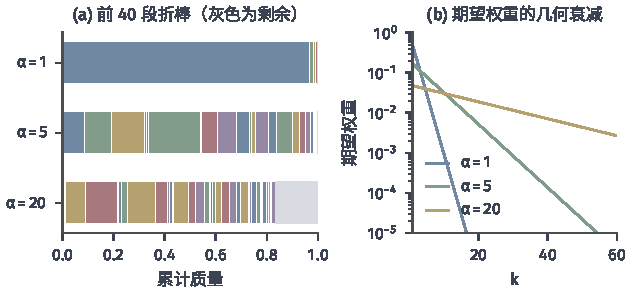
\includegraphics[width=107mm]{figures/03-optimization-evolution-and-signals/02-processes-and-trajectory-evolution/matplotlib/spp-stick-breaking/figure.pdf}
  \caption{折棒构造$w_1=V_1$，$w_k=V_k\prod_{j<k}(1-V_j)$，$V_k$独立服从$\operatorname{Beta}(1,\alpha)$。(a)$\alpha=1,5,20$各一次实现的前$40$段（颜色循环只用于区分相邻段，固定随机种子），灰色为前$40$段之后的剩余质量。(b)期望权重$\mathbb Ew_k=(1+\alpha)^{-1}\bigl(\alpha/(1+\alpha)\bigr)^{k-1}$（对数纵轴）。}
  \label{fig:spp-stick-breaking}
\end{figure}

首先要确认折下的各段加起来确实是整根木棒。记剩余长度$R_n=\prod_{j\le n}(1-V_j)$。由归纳，$\sum_{k\le n}w_k=1-R_n$：$n=1$时成立，且$1-R_n+w_{n+1}=1-R_n+V_{n+1}R_n=1-R_{n+1}$。

\begin{lemma}[剩余质量趋于零]
\label{lem:spp-stick-remainder}
$R_n\to0$几乎必然成立，从而$\sum_{k\ge1}w_k=1$几乎必然成立。
\end{lemma}

\begin{proof}
$R_n$非负且关于$n$不增，几乎必然收敛到某个$R_\infty\ge0$。由独立性，$\mathbb ER_n=\prod_{j\le n}\mathbb E(1-V_j)=\bigl(\alpha/(1+\alpha)\bigr)^n$。又$R_\infty\le R_n$，所以$\mathbb ER_\infty\le\bigl(\alpha/(1+\alpha)\bigr)^n$对每个$n$成立，$\mathbb ER_\infty=0$。非负随机变量的期望为零，它几乎必然为零。
\end{proof}

在$\sum_kw_k=1$的事件上按式~\eqref{eq:spp-random-discrete}定义$G$，在其补集这个零概率事件上令$G=G_0$。由上一小节，这样得到的$G$是随机概率测度，并且每次实现都是概率测度。

\paragraph{有限分割的Dirichlet规律}
剩下要证明折棒构造给出的$G$确实是Dirichlet过程。证明的想法来自一个自相似性：折下第一段后，剩下的部分按同样的规则继续折，所以$G$等于“一个原子的质量$V_1$”加上“比例为$1-V_1$的一个同分布的随机测度”。若Dirichlet分布在这一操作下保持不变，再加上剩余质量趋于零，就能推出结论。这一构造由Sethuraman提出。

\begin{theorem}[折棒构造给出Dirichlet过程]
\label{thm:spp-stick-breaking-dp}
设$V_k$独立服从$\operatorname{Beta}(1,\alpha)$，$\xi_k$独立同分布于$G_0$且与$(V_k)$独立，$G$由式~\eqref{eq:spp-stick-breaking}与式~\eqref{eq:spp-random-discrete}定义（在零概率例外事件上令$G=G_0$）。则$G\sim\operatorname{DP}(\alpha,G_0)$。
\end{theorem}

\begin{proof}
固定有限可测分割$(A_1,\ldots,A_K)$，记$g_i=G_0(A_i)$。若某个$g_i=0$，则几乎必然没有原子落入$A_i$，$G(A_i)=0$，符合零参数的约定；删去这些分块后，不妨设所有$g_i>0$，$K\ge2$（$K=1$时结论平凡）。令$J_k$为$\xi_k$所在分块的编号，则$J_1,J_2,\ldots$独立同分布，$\mathbb P(J_k=i)=g_i$，且与$(V_k)$独立。记$\bm e_i$为第$i$个标准单位向量，质量向量可以写成
\[
  \bm P=\bigl(G(A_1),\ldots,G(A_K)\bigr)=\sum_{k\ge1}w_k\bm e_{J_k}.
\]
记$\bm g=(g_1,\ldots,g_K)$，目标是证明$\bm P\sim\operatorname{Dir}(\alpha\bm g)$。

第一步，一步不变性：若$\bm Q\sim\operatorname{Dir}(\alpha\bm g)$，$V\sim\operatorname{Beta}(1,\alpha)$，$J$以概率$g_i$取$i$，三者独立，则$V\bm e_J+(1-V)\bm Q\sim\operatorname{Dir}(\alpha\bm g)$。先固定$J=i$。取相互独立的$Y_0$（Gamma参数$1$）与$Y_1,\ldots,Y_K$（Gamma参数$\alpha g_1,\ldots,\alpha g_K$），令$\Sigma=\sum_{l\ge1}Y_l$。由引理~\ref{lem:spp-gamma-normalization}，$(Y_l/\Sigma)_l\sim\operatorname{Dir}(\alpha\bm g)$且与$\Sigma$独立，也与$Y_0$独立；$\Sigma$的参数为$\alpha$，所以$Y_0/(Y_0+\Sigma)\sim\operatorname{Beta}(1,\alpha)$，并且它与$(Y_l/\Sigma)_l$独立。于是$(V,\bm Q)$与$\bigl(Y_0/(Y_0+\Sigma),(Y_l/\Sigma)_l\bigr)$同分布，
\[
  V\bm e_i+(1-V)\bm Q\overset{\mathrm d}{=}\frac{Y_0\bm e_i+(Y_1,\ldots,Y_K)}{Y_0+\Sigma}\sim\operatorname{Dir}(\alpha\bm g+\bm e_i),
\]
因为第$i$个分子$Y_0+Y_i$服从参数为$\alpha g_i+1$的Gamma分布，且各分子仍独立。再对$J$平均。由引理中的密度，并利用$\Gamma(\alpha+1)=\alpha\Gamma(\alpha)$与$\Gamma(\alpha g_i+1)=\alpha g_i\Gamma(\alpha g_i)$，$\operatorname{Dir}(\alpha\bm g+\bm e_i)$的密度等于$\operatorname{Dir}(\alpha\bm g)$的密度$D(\bm p)$乘以$\frac{\alpha}{\alpha g_i}p_i=p_i/g_i$。所以混合的密度为
\[
  \sum_{i=1}^Kg_i\cdot\frac{p_i}{g_i}D(\bm p)=\Bigl(\sum_ip_i\Bigr)D(\bm p)=D(\bm p),
\]
即$V\bm e_J+(1-V)\bm Q\sim\operatorname{Dir}(\alpha\bm g)$。

第二步，有限步迭代。取$\bm Q_0\sim\operatorname{Dir}(\alpha\bm g)$，与全部$(V_k,J_k)$独立，令
\[
  \bm P^{(n)}=\sum_{k\le n}w_k\bm e_{J_k}+R_n\bm Q_0 .
\]
它可以写成$\bm P^{(n)}=V_1\bm e_{J_1}+(1-V_1)\bm P'^{(n-1)}$，其中$\bm P'^{(n-1)}$是用$(V_2,\ldots,V_n)$、$(J_2,\ldots,J_n)$与$\bm Q_0$按同样公式构成的向量，与$(V_1,J_1)$独立。对$n$归纳：$\bm P^{(0)}=\bm Q_0\sim\operatorname{Dir}(\alpha\bm g)$；若$n-1$步的向量服从$\operatorname{Dir}(\alpha\bm g)$，则$\bm P'^{(n-1)}$也服从它，由第一步，$\bm P^{(n)}\sim\operatorname{Dir}(\alpha\bm g)$。

第三步，取极限。在$\sum_kw_k=1$的事件上，$\bm P-\bm P^{(n)}=\sum_{k>n}w_k\bm e_{J_k}-R_n\bm Q_0$，每个坐标的绝对值不超过$\sum_{k>n}w_k+R_n=2R_n$。由引理~\ref{lem:spp-stick-remainder}，$\bm P^{(n)}\to\bm P$几乎必然成立，从而依分布收敛；而每个$\bm P^{(n)}$的分布都是$\operatorname{Dir}(\alpha\bm g)$，所以$\bm P\sim\operatorname{Dir}(\alpha\bm g)$。
\end{proof}

\paragraph{浓度参数与基测度的作用}
由Beta边缘的均值与方差公式，对每个可测集$A$，
\[
  \mathbb EG(A)=G_0(A),\qquad \operatorname{Var}G(A)=\frac{G_0(A)\bigl(1-G_0(A)\bigr)}{1+\alpha}.
\]
基测度$G_0$决定随机测度的平均形状，浓度参数$\alpha$决定它围绕平均形状的离散程度。图~\ref{fig:spp-dp-samples}以$G_0=\mathcal N(0,1)$画出随机分布函数$G((-\infty,x])$的样本：$\alpha=1$时，几个大原子造成少数几级大台阶，样本与$G_0$相去甚远；$\alpha=100$时，样本紧贴$G_0$的分布函数。

\begin{figure*}[htbp]
  \centering
  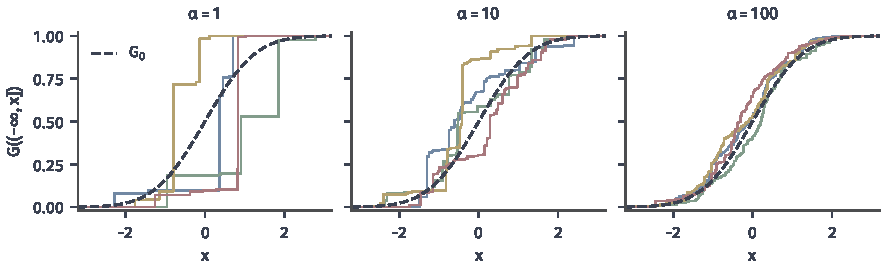
\includegraphics[width=150mm]{figures/03-optimization-evolution-and-signals/02-processes-and-trajectory-evolution/matplotlib/spp-dp-samples/figure.pdf}
  \caption{Dirichlet过程$\operatorname{DP}(\alpha,\mathcal N(0,1))$的随机分布函数$x\mapsto G((-\infty,x])$。每幅图画四次独立实现（彩色阶梯线，由折棒构造截断到$6000$个原子生成，截断后剩余质量可忽略，固定随机种子），虚线为基测度$\mathcal N(0,1)$的分布函数。浓度参数从左到右为$\alpha=1,10,100$。}
  \label{fig:spp-dp-samples}
\end{figure*}

无论$G_0$是否连续，折棒构造的每次实现都是离散测度。这在抽样时有一个直接后果。给定$G$，独立抽取$X_1,X_2\sim G$；若$G_0$没有原子，则不同的$\xi_k$几乎必然互不相同，$X_1=X_2$当且仅当两次抽到同一个原子，于是
\[
  \mathbb P(X_1=X_2)=\mathbb E\sum_kw_k^2=\frac1{1+\alpha}.
\]
最后一个等式的计算如下：$\mathbb EV^2=2/\bigl((1+\alpha)(2+\alpha)\bigr)$，$\mathbb E(1-V)^2=\alpha/(2+\alpha)$，由独立性
\[
  \mathbb E\sum_kw_k^2=\mathbb EV^2\sum_{k\ge1}\bigl(\mathbb E(1-V)^2\bigr)^{k-1}=\frac{2}{(1+\alpha)(2+\alpha)}\cdot\frac{2+\alpha}2=\frac1{1+\alpha}.
\]
$\alpha$越小，重复抽到同一个值的概率越大。由de Finetti定理的反向结论，给定$G$后条件独立抽取的$X_1,X_2,\ldots$构成一个可交换序列，它的随机背景$\Xi$就是$G$；这把本节与上一节连在一起。这种重复取值的结构是Dirichlet过程用于聚类的出发点。

有限Dirichlet分布族的系统性质由卷四的概率分布部分处理；给定观测后Dirichlet过程的后验、由重复取值导出的聚类表示以及非参数推断，则由卷四的统计推断部分处理。
